\chapter{The Semantic Pointer Architecture}\label{sec:spa}
While the Neural Engineering Framework allows us to encode vectors into spiking neural networks and transform them, it does not tell us how to use those vectors to represent structured, conceptual, or symbol-like information.
Different such methods could be devised, though in the context of the NEF the most widely used method is the Semantic Pointer Architecture \parencite[SPA;][]{eliasmith2013}.
The SPA has been used to build a multitude of cognitive models, including the n-back task \parencite{gosmann2015}, the Tower of Hanoi task \parencite{stewart2011-2}, human-scale knowledge representation \parencite{crawford2016}.
The largest and most complex example of a SPA model is Spaun, the Semantic Pointer Architecture Unified Network, combining eight different tasks in a single functional spiking-neuron model \parencite{Eliasmith2012}.

The conceptual representations in the SPA are a specific instance of a Vector Symbolic Architecture \parencite[VSA;][]{gayler2004}.
In VSAs concepts are represented with vectors, and linear and nonlinear operators are used to combine basic concepts in more complex structured representations.
Three types of operators are considered essential in a VSA\@.
First, a measure of similarity
\begin{equation}
    \simmeasure: \mathbb{R}^{\dims} \times \mathbb{R}^{\dims} \longrightarrow \mathbb{R}
\end{equation}
for which I use the normalized dot product (also known as cosine similarity)
\begin{equation}
    \simmeasure(\vc x, \vc y) := \frac{\left\langle \vc x, \vc y \right\rangle}{\norm{\vc x} \cdot \norm{\vc y}}
\end{equation}
for the remainder of this thesis.
Second, a superposition operator
\begin{equation}
    \superpos: \mathbb{R}^{\dims} \times \mathbb{R}^{\dims} \longrightarrow \mathbb{R}^{\dims}
\end{equation}
is required that produces a vector similar to both inputs, i.e., $\simmeasure(\superpos(\vc x, \vc y), \vc x) \approx \simmeasure(\superpos(\vc x, \vc y), \vc y) \gtrapprox \sqrt{1/2}$ for $\simmeasure(\vc x, \vc y) \approx 0$.
This is usually, and will be for the remainder of this thesis, simple elementwise addition, i.e., $\superpos(\vc x, \vc y) := \vc x + \vc y$.
Finally, a binding operator
\begin{equation}
    \bind: \mathbb{R}^{\dims_1} \times \mathbb{R}^{\dims_2} \longrightarrow \mathbb{R}^{\dims}
\end{equation}
is needed with an approximate inverse or unbinding operation
\begin{equation}
    \bind^+: \mathbb{R}^d \times \mathbb{R}^{\dims_2} \longrightarrow \mathbb{R}^{\dims_1} \text{.}
\end{equation}
To be able to build up and retrieve information from representations, the binding and unbinding operations are required to be distributive, i.e.,
\begin{align}
    \bind(\vc x + \vc y, \vc z) &= \bind(\vc x, \vc z) + \bind(\vc y, \vc z) \\
    \bind^+(\vc x + \vc y, \vc z) &= \bind^+(\vc x, \vc z) + \bind^+(\vc y, \vc z) \text{.}
\end{align}

For some proposed binding operations, like Tensor products \parencite{smolensky1990}, the unbinding operation is the exact inverse $\bind^+ = \bind^{-1}$ with
\begin{equation*}
    \bind^{-1}(\bind(\vc x, \vc y), \vc y) = \vc x \text{.}
\end{equation*}
However, Tensor products increase the vector dimensionality with each successive binding which leads to biological implausible scaling problems \parencite[Appendix D.5]{eliasmith2013}.
For that reason, I will only consider binding methods that keep the dimensionality $\dims = \dims_1 = \dims_2$ constant.

In pure math, it is still possible to define binding operators with an exact inverse, but we need to keep the implementation in neurons in mind.
This introduces additional constraints.
First, the actual usable representational space $\repspace \subsetneq \mathbb{R}^{\dims}$ is limited, constraining unlimited growth of bound vectors.
Second, neural noise limits the representational accuracy, preventing highly non-linear operators.
It follows that for a binding operator in a neural system it is desired to maximize the set $\mathcal{V} \subseteq \repspace$ for which  $\simmeasure(\bind^+(\bind(\vc x, \vc y) + \vc\zeta, \vc y), \vc x) \approx 1$ for all $\vc x, \vc y \in \mathcal{V}$ and samples of noise $\vc\zeta$ in the neural system.
Note that this condition would be satisfied by using the identity $\bind(\vc x, \vc y) = \bind^+(\vc x, \vc y) = \vc x$.
Thus, simultaneously it needs to hold that $\simmeasure(\bind^+(\bind(\vc x, \vc y), \vc z), \vc x) \approx 0$ for all $\vc x, \vc y, \vc z \in \mathcal{V}$ with $\simmeasure(\vc y, \vc z) \approx 0$.
At this point, it is useful to introduce three more definitions.

\begin{defn}[identity vector]
    A vector $\bid_{\bind}$ with the property $\bind(\vc x, \bid_{\bind}) = \vc x$ is called \emph{identity vector} under $\bind$.
\end{defn}
\begin{defn}[absorbing element]
    A vector $\bzero_{\bind}$ with the property $\bind(\vc x, \bzero_{\bind}) = c \cdot \bzero_{\bind}$ where $c \in \mathbb{R}$ is called an \emph{absorbing element} under $\bind$.
\end{defn}
Such an absorbing element effectively destroys the information in the vector $\vc x$.
For that reason, absorbing elements should be avoided when constructing representations with binding.
Note that this definition slightly differs from the usual definition of absorbing elements by allowing for a scaling factor.
\begin{defn}[unitary vector]
    A vector $\vc u$ with the property $\langle \bind(\vc x, \vc u), \bind(\vc y, \vc u) \rangle = \langle \vc x, \vc y \rangle$ is called unitary.
\end{defn}
In other words, a unitary vector preserves the dot product under binding.
This is in analogy to unitary transformation matrices that also preserve the dot product.
It also implies that binding with a unitary vector preserves the length of the bound vector.


\section{Binding operations}
I introduce two specific binding operations now.
First, circular convolution is discussed, which has been the binding operation of choice in the SPA so far.
Second, I introduce a new binding method, termed vector-derived transformation binding, with some trade-offs.
The two binding approaches and their suitability for different problems is discussed.

\subsection{Circular convolution}
The binding operator classically used in the SPA is circular convolution, and was suggested by \textcite{plate1995,plate2003} for his Holographic Reduced Representations (HRRs).
\begin{defn}[circular convolution binding]
    The circular convolution binding operator is given by
    \begin{equation}
        \bind_{\circledast}(\vc x, \vc y) := \vc x \circledast \vc y\ \text{with}\ \del{\vc x \circledast \vc y}_i = \sum_{j=0}^{d - 1} x_j y_{(i - j) \bmod d}
    \end{equation}
    and has the approximate inverse \parencite{plate2003}
    \begin{equation}
        \bind^+_{\circledast}(\vc x, \vc y) = \vc x \circledast \vc y^+\ \text{with}\ \vc y^+ := \del{y_0, y_{d-1}, y_{d-2}, \dotsc, y_1}\Tr \text{.}
    \end{equation}
\end{defn}

The basic properties of
\begin{align}
    &\text{distributivity:} &(\vc x_1 + \vc x_2) \circledast \vc y &= \vc x_1 \circledast \vc y + \vc x_2 \circledast \vc y \text{,}\\
    &\text{associativity:} &(\vc x \circledast \vc y) \circledast \vc z &= \vc x \circledast (\vc y \circledast \vc z) \text{,} \\
    &\text{commutativity:} &\vc x \circledast \vc y &= \vc y \circledast \vc x
\end{align}
hold for circular convolution as a binding operator.
A useful property of circular convolution for the implementation in a neural network with the NEF is, that it becomes element-wise multiplication in the Fourier space defined by
\begin{equation}
    \vc x \circledast \vc y = \fouriermat^{-1}\sbr{(\fouriermat \vc x) \circ (\fouriermat \vc y)}
\end{equation}
where $\fouriermat$ is the discrete Fourier transform (DFT) matrix.
The linear transform with the DFT matrix can be put easily into the neural connection weights and the element-wise product can be done with a well-optimized product network \parencite{gosmann2015-1}.

The expression in Fourier space also allows the derivation of the special elements of circular convolution.
The identity vector must not change the complex Fourier coefficient in the element-wise multiplication.
Thus, its Fourier coefficients must all be $1 + 0\iu$ and the identity vector is given by
\begin{equation}
    \bid_{\circledast} = (1, 0, 0, \dotsc, 0)\Tr \text{.}
\end{equation}
Furthermore, all vectors with Fourier coefficients $c_n \in \mathbb{C}$ that have an absolute value of $\left|c_n\right| = 1$ will be unitary, as one can easily verify.
A trivial example of a unitary vector is the identity vector $\bid_{\circledast}$.
Finally, all vectors $(z, \dotsc, z)\!\Tr$ with $z \in \mathbb{R}$ are absorbing elements.

\subsection{Vector-derived transformation binding}
Circular convolution can be interpreted as moving one of the operands around in the $d$-dimensional space in a way defined by the other operand.
This leads to the question, whether there are other ways to project one vector to a new location based on the other vector.
One such way is what I call \emph{vector-derived transformation binding (VTB)}, which to my knowledge has not been described before.
\begin{defn}[vector-derived transformation binding, VTB]
    Given a $\dims' = \dims^{\frac{1}{2}} \in \posnum$, the vector-derived transformation binding operator $\vtb: \mathbb{R}^{\dims} \times \mathbb{R}^{\dims} \longrightarrow \mathbb{R}^{\dims}$ is defined as
    \begin{equation}
        \vtb(\vc x, \vc y) := \bar{\mat V}_{\vc y} \vc x = \begin{bmatrix}
            \mat V_{\vc y} & 0 & 0 \\
            0 & \mat V_{\vc y} & 0 \\
            0 & 0 & \ddots
        \end{bmatrix} \vc x
    \end{equation}
    with
    \begin{equation}
        \mat V_{\vc y} = \dims^{\frac{1}{4}} \begin{bmatrix}
            y_1 & y_2 & \dotso & y_{\dims'} \\
            y_{\dims' + 1} & y_{\dims' + 2} & \dotso & y_{2\dims'} \\
            \vdots & \vdots & \ddots & \vdots \\
            y_{\dims - \dims' + 1} & y_{d - \dims' + 2} & \dotso & y_{\dims}
        \end{bmatrix} \text{.}
    \end{equation}
    The approximate inverse is given by
    \begin{equation}
        \vtb^+(\vc x, \vc y) = \bar{\mat V}_{\vc y}\Tr \vc x = \begin{bmatrix}
            V_{\vc y}\Tr & 0 & 0 \\
            0 & V_{\vc y}\Tr & 0 \\
            0 & 0 & \ddots
        \end{bmatrix} \vc x \text{.}
    \end{equation}
\end{defn}
This binding method is based on the fact that in the SPA vectors are usually randomly generated and uniformly distributed with identically distributed components.
In that case each subvector (e.g., each row in $\mat V_{\vc y}$) is also uniformly distributed with identically distributed components.
Furthermore, for high-dimensional vector spaces almost all (uniformly sampled) vectors are orthogonal and semantic pointers are usually picked to have unit-length.
Thus, the matrix $\bar{\mat V}_{\vc y}$ is almost orthogonal with the implication $\bar{\mat V}_{\vc y}\Tr \bar{\mat V}_{\vc y} \approx \imat$.
Vectors $\vc y$ that give a perfectly orthogonal matrix $\mat V_{\vc y}$, will be unitary.
One special unitary vector is the identity vector.
\begin{corollary}[VTB identity vector]
    The identity vector for VTB is given by
    \begin{equation}
        \sbr{\bid_{\ped{V}}}_i = \left\{ \begin{array}{ll}
                \dims^{-\frac{1}{4}} & i \in \cbr{(k - 1) \dims' + k : k \leq \dims', k \in \mathbb{N}_{>0}} \\
                0 & \text{otherwise}
        \end{array}\right. \text{.}
    \end{equation}
    \begin{proof}
        By writing $\bid_{\ped{V}}$ as $\mat V_{\bid_{\ped{V}}}$ one can easily verify that $\mat V_{\bid_{\ped{V}}} = \imat\ \Rightarrow\ \bar{\mat V}_{\bid_{\ped{V}}} = \imat$.
    \end{proof}
\end{corollary}
Example for $d = 9$: $\bid_{\ped{V}}^{(9)} = (1, 0, 0, 0, 1, 0, 0, 0, 1)\Tr$.

\begin{corollary}[VTB distributivity]
    VTB is distributive:
    \begin{equation}
        \begin{split}
            \vtb(\vc x_1 + \vc x_2, \vc y) &= \vtb(\vc x_1, \vc y) + \vtb(\vc x_2, \vc y) \text{ and}\\
            \vtb(\vc x, \vc y_1 + \vc y_2) &= \vtb(\vc x, \vc y_1) + \vtb(\vc x, \vc y_2) \text{.}
        \end{split}
    \end{equation}
    \begin{proof}
        By applying the definitions for both directions of the distributivity:
        \begin{itemize}
            \item $\vtb(\vc x_1 + \vc x_2, \vc y) = \bar{\mat V}_{\vc y} \del{\vc x_1 + \vc x_2} = \bar{\mat V}_{\vc y} \vc x_1 + \bar{\mat V}_{\vc y} \vc x_2 = \vtb(\vc x_1, \vc y) + \vtb(\vc x_2, \vc y)$
            \item $\vtb(\vc x, \vc y_1 + \vc y_1) = \bar{\mat V}_{\vc y_1 + \vc y_2} \vc x = \del{\bar{\mat V}_{\vc y_1} + \bar{\mat V}_{\vc y_2}} \vc x = \bar{\mat V}_{\vc y_1} \vc x + \bar{\mat V}_{\vc y_2} \vc x = \vtb(\vc x, \vc y_1) + \vtb(\vc x, \vc y_2)$
    \end{itemize}
    \end{proof}
\end{corollary}
In contrast to circular convolution, VTB is neither commutative
\begin{equation}
    \vtb(\vc x, \vc y) = \bar{\mat V}_{\vc y} \vc x \neq \bar{\mat V}_{\vc x} \vc y = \vtb(\vc y, \vc x) \text{,}
\end{equation}
nor associative
\begin{equation}
    \vtb(\vc x, \vtb(\vc y, \vc z)) = \bar{\mat V}_{\bar{\mat V}_{\vc z} \vc y} \vc x \neq \bar{\mat V}_{\vc z} \bar{\mat V}_{\vc y} \vc x = \vtb(\vtb(\vc x, \vc y), \vc z) \text{.}
\end{equation}
This implies that unlike circular convolution, multiple bindings cannot be undone in a single step, but a separate unbinding step is required for each binding.
Despite the non-commutativity, it is possible to flip the operands in the bound state $\vtb(\vc x, \vc y) = \mat V_{\leftrightarrow} \vtb(\vc y, \vc x)$ with the matrix
\begin{equation}
    \sbr{\mat V_{\leftrightarrow}}_{ij} = \left\{ \begin{array}{ll}
            1 & j = 1 + \left\lfloor \frac{i - 1}{\dims'} \right\rfloor + \dims' \sbr{\del{i - 1} \bmod \dims'} \\
            0 & \text{otherwise}
        \end{array}\right. \text{.}
\end{equation}
Example for $d = 4$:
\begin{equation*}
    \mat V_{\leftrightarrow}^{(4)} = \sbr{\begin{array}{cccc}
            1 & 0 & 0 & 0 \\
            0 & 0 & 1 & 0 \\
            0 & 1 & 0 & 0 \\
            0 & 0 & 0 & 1
        \end{array}}
\end{equation*}

\subsection{Comparison of circular convolution and vector-derived transformation binding}
Both circular convolution and VTB are compressed binding operations.
Because of the lossy compression, we lose some information in each binding which makes it increasingly harder to recover the original unbound vectors.
To combat this effect (and the effect of neuron noise) clean-up memories like the one by \textcite{stewart2011} are required.
Likewise the independent accumulator model discussed in \cref{sec:ia} can be used as a clean-up memory.

In addition to the information loss, the binding operations change the length of the vector (if neither operand is unitary).
This can be a problem in a neural representation as neurons saturate and might not represent the vector accurately anymore.
In particular, neural ensembles in the NEF are optimized for a certain representational space, usually a hyperball with a given radius $\radius$.
It is convenient to set $\radius = 1$ and try to keep the Semantic Pointer vectors at unit-length.

\Cref{fig:bindings-autoconv} shows how the mean length of random vectors repeatedly bound with themselves changes.
For the circular convolution the length increases much faster than for VTB\@.
Such a rapid increase in length can be problematic in a neural network with a limited representational radius as in the NEF\@.
Moreover, VTB preserves more information of the bound vectors as shown by the similarity to the original vectors when undoing all bindings.
After repeated binding with itself and then the same number of unbindings, the resulting VTB bound vector is more similar to the original vector than the circular convolution bound vector.
\begin{figure}
    \centering
    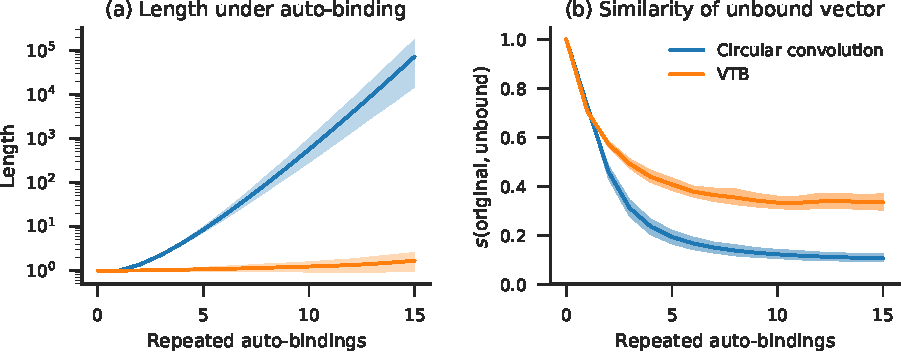
\includegraphics{figures/bindings-autoconv}
    \caption[Repeatedly binding a 256-dimensional vector with itself]{Repeatedly binding a 256-dimensional vector with itself. (a) Length of the resulting vector. (b) Similarity of the original vector to the vector obtained when undoing all bindings. The shaded areas represent \SI{95}{\percent} confidence intervals.}\label{fig:bindings-autoconv}
\end{figure}

While binding vectors with themselves can sometimes be useful (e.g., for generating Semantic Pointers with a successive relationship like position indices), it is much more common to bind randomly sampled vectors.
\Cref{fig:bindings-random} shows the same experiment where a random vector was used in each binding.
In this case, the vector length will decrease to zero, even if it might increase in some of the early bindings.
Again, this decrease is much quicker for circular convolution binding than for VTB and the latter method also preserves more of the similarity across bindings.
\begin{figure}
    \centering
    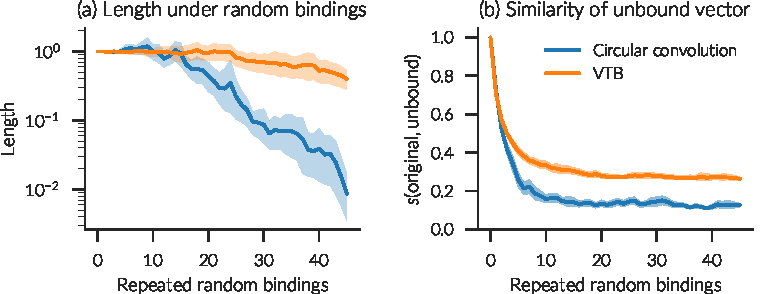
\includegraphics{figures/bindings-random}
    \caption[Repeatedly binding a 256-dimensional vector with random vectors]{Repeatedly binding a 256-dimensional vector with random vectors. (a) Length of the resulting vector. (b) Similarity of the original vector to the vector obtained when undoing all bindings. The shaded areas represent \SI{95}{\percent} confidence intervals.}\label{fig:bindings-random}
\end{figure}

It is conceivable that the problems with scaling of the vector length can be fixed by normalizing after each binding.
This, however, does not affect the loss of information in each binding (\cref{fig:bindings-normalized}).
Also, implementing normalization in a neural network is notoriously difficult because of the division involved with an unbounded output as the divisor approaches zero.
Good approximations of normalization are only possible for a defined and finite input range.
It is worth noting that the neurons in the NEF perform a sort of ``soft normalization'' for large values, as the neuron's firing rates saturate.
But this only affects vectors exceeding a certain length and can lead to other distortions in the representation.
\begin{figure}
    \centering
    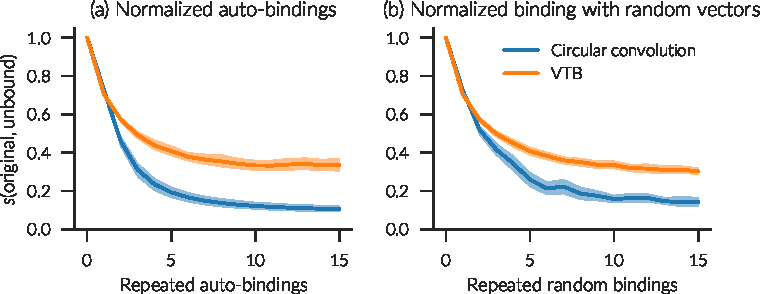
\includegraphics{figures/bindings-normalized}
    \caption[Repeatedly binding a 256-dimensional vector with normalization]{Repeatedly binding a 256-dimensional vector with (a) itself or (b) random vectors and normalizing in each step. The similarity to the original vector after undoing all bindings is shown. The shaded areas represent \SI{95}{\percent} confidence intervals.}\label{fig:bindings-normalized}
\end{figure}

Another approach to preventing the growth or decay of the vector length, and even prevent the information loss, is the usage of unitary vectors.
These keep the vector length constant and perform lossless binding due to their perfect inverse.
Note that binding two unitary vectors gives another unitary vector.
Thus, repeated binding is not a problem.
However, the scaling properties of VSAs are based on the fact that the number of almost orthogonal vectors that fits into a vector space grows exponentially with the dimensionality of that space \parencite{wyner1967,cai2013}.
Because not all vectors are unitary, this scaling property might be lost when restricted to unitary vectors.
It might be best to use unitary vectors only for those Semantic Pointers that are repeatedly used in bindings.
But it is also worth keeping in mind that achieving the theoretical limit of almost orthogonal vectors in a space is a hard problem, closely related to sphere packing and unsolved for arbitrary dimensionality \parencite{cohn2017}.
Thus, the practical scaling of the number of useable vectors might be less then the exponential scaling for both unitary and non-unitary vectors.

So far VTB looks like the better choice for a binding operation.
But it does not come not without downsides.
In contrast to circular convolution, it is not associative or commutative.
While the desirability of commutativity depends on the employed representation scheme, the non-associativity implies that each binding has to be undone in an individual step, while circular convolution allows us to undo a chain of bindings in a single step, if the vector representing that chain is available.
Thus, circular convolution can allows the recovery of information more quickly.
Ultimately, this is a question of what binding operations the brain applies for different forms of processing (if such binding is at all related to what the brain does).
Potentially, the binding operations lead to different timing predictions, as unbinding with the VTB may take more time.
Deriving such predictions and testing them experimentally is, however, out of the scope of this thesis.

Finally, we have to consider the neural implementation of these binding operations.
Both essentially require a set of multiplication networks.
For the circular convolution, the DFT (and inverse DFT) can be implemented in feed-forward connection weights that do not require any additional neurons.
For each of the input vectors $\dims$ Fourier complex coefficients will be produced, but as the inputs are real-valued, half of these are the complex conjugate of the other half.
Thus, only $\dims / 2$ coefficients have to be considered.
Each coefficient is a complex number multiplied with one coefficient of the other vector.
That results in four real-valued multiplies per coefficient.
In total, $2\dims$ multiplications are required for a circular convolution.
For VTB, there are $d^{1/2}$ multiplications of $d^{1/2} \times d^{1/2}$ matrices with a vector, resulting in a total of $d^{3/2}$ multiplications.
Thus, the VTB requires more neural resources as a larger number of multiplication networks is required.
It should be noted, that for either binding method, the binding with a fixed vector can be implemented purely in the connection weights as it reduces to a simple matrix multiplication in either case.

Despite VTB having many advantages over circular convolution, I decided to use circular convolution in the memory model.
The main reason is that support for circular convolution is already implemented in Nengo and the model does not use a lot of binding operations.
Nevertheless, it would be interesting to switch the model over to VTB and investigate effects on the performance in the future.


\section{Structured representations}
Once we defined a binding operation, it can be used to build up structured representations with Semantic Pointers.
For example, consider a scene with a red square and blue circle that we want to encode as Semantic Pointer.
Assume that we have Semantic Pointers \spc{red}, \spc{square}, \spc{blue}, and \spc{circle}.
One possible encoding would be
\begin{equation}
    \vc s = \bind(\spc{red}, \spc{square}) + \bind(\spc{blue}, \spc{circle}) \text{.}
\end{equation}
We could then recover the color of the square as
\begin{align}
    \bind^+(\vc s, \spc{color}) &= \bind^+(\bind(\spc{red}, \spc{square}), \spc{square}) + \bind^+(\bind(\spc{blue}, \spc{circle}), \spc{square}) \\
    &\approx \spc{red} + \mathrm{noise} \text{.}
\end{align}
Note, however, that the binding operation needs to be commutative to recover the shape from the color with this encoding scheme.
Other encoding schemes can be devised to alleviate this concern.
For example, the properties can be bound to a role and each object to an object identifier:
\begin{align}
    \vc o_1 &= \bind(\spc{red}, \spc{color}) + \bind(\spc{square}, \spc{shape}) \\
    \vc o_2 &= \bind(\spc{blue}, \spc{color}) + \bind(\spc{circle}, \spc{shape}) \\
    \vc s &= \bind(\vc o_1, \spc{obj}_1) + \bind(\vc o_2, \spc{obj}_2) \text{.}
\end{align}
To find the color of a specific shape, each object would have to be retrieved, then the shape of the object to compare it to the target shape, and finally the color has to recovered if the shape matches.
Thus, different encoding schemes can lead to different timing predictions.
The latter approach requires scanning and through multiple objects and thus it should take longer to recover information with more items, while the former approach can recover any property in a single step.
Despite those differences, both encoding approaches are similar, in so far as pairs of semantic pointers are bound together.
\begin{defn}[encoding with binding]
    Given $k$ pairs $(\vc x_i, \vc y_i) \in \mathbb{R}^{\dims} \times \mathbb{R}^{\dims}$, the encoding of these pairs into a single Semantic Pointer $\vc m$ with binding is given by
    \begin{equation}
        \vc m = \sum_{i=1}^k \bind(\vc x_i, \vc y_i) \text{.}
    \end{equation}
\end{defn}
An $\vc x_i$ from such a trace can be recalled as $\vc x_i \approx \hat{\vc x}_i = \bind^+(\vc m, \vc x_i)$.
While most concrete encoding schemes make use of encoding with binding, at least one other method, encoding with tagging, has been proposed \parencite{recchia2015}.
\begin{defn}[encoding with tagging]
    Given $k$ pairs $(\vc x_i, \vc y_i) \in \mathbb{R}^{\dims} \times \mathbb{R}^{\dims}$ and a matrix $\mat M \in \mathbb{R}^{\dims \times \dims}$ with an approximate inverse $\mat M^+$ satisfying $\mat M^+ \mat M \approx \imat$, the encoding into a single Semantic Pointer with tagging is given by
    \begin{equation}
        \vc m = \sum_{i=1}^k \mat M^{2i-1} \del{\vc y_i + \mat M \vc x_i} = \sum_{i=1}^k \mat M^{2i-1} \vc y_i + \mat M^{2i} \vc x_i \text{.}
    \end{equation}
\end{defn}
The retrieval of an $\vc x_i \approx \hat{\vc x}_i$ is accomplished with
\begin{align}
    \hat{\vc x}_i &:= \del{\mat M^{2c}}^+ \vc m \\
    c &= \argmax_{j \in \sbr{1, k}}\ \simmeasure\!\del{\vc y_i, \del{\mat M^{2j-1}}^{\!+} \vc m} \text{.}
\end{align}

There are a number of sensible choices for the matrix $\mat M$.
\begin{itemize}
    \item First of all, for both, circular convolution and VTB, binding with a \emph{fixed} vector $\vc v$ can be expressed as a matrix multiplication.
        A matrix $\mat M$ derived in this way is unitary, if and only if the vector $\vc v$ is unitary for the given binding operation.
    \item A common choice for encoding with tagging are permutation matrices.
        These are unitary and an exact inverse is given by the transpose.
    \item A special permutation matrix is the matrix that shifts all vector components by one.
        For a given permutation matrix, the vector space dimensions can be reordered such that the permutation matrix becomes the shift by one.
        Interestingly, the shift by one is also equivalent to a circular convolution with the vector $(0, 1, 0, 0, \dotsc)\Tr$.
    \item Other good candidates for $M$, that have not been considered to my knowledge, are (random) orthogonal matrices.
        These are unitary operators on $\mathbb{R}^{\dims}$ and thus have an exact inverse given by the transpose.
\end{itemize}
The relations of these different matrix choices is shown in the Venn diagram in \cref{fig:tagging-matrices}.
\begin{figure}
    \centering
    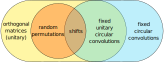
\includegraphics{figures/tagging-matrices}
    \caption[Venn diagram of matrices for encoding with tagging]{Venn diagram of the relations between different classes of matrices $\mat M$ that can be used for encoding with tagging.}\label{fig:tagging-matrices}
\end{figure}

Either encoding method allows the recovery of encoded vectors, but the encoding vector itself is (in general) not similar to those encoded vectors.
In this way, the vector is analogous to a pointer in computer science that doesn't directly contain the information, but can be dereferenced to access the information it is pointing to.
Unlike pointers, however, these vectors can also capture semantic information by their distance in vector space.
Due to the combination of these two facts, these vectors are called Semantic Pointers. 


\subsection{Comparison of encoding methods}
Based on experiment~1 from \textcite{recchia2015}, the encoding methods can be compared by measuring the pairwise binding capacity.
To do so, a set of \num{1000}~vectors with normally distributed components $x_i \sim \ndist\!\del{\!0, \sqrt{1/\dims}}$ are created (note that $\expected\!\sbr{\,\norm{\vc x}} = 1$).
From this set \num{500}~pairs are sampled with replacement.
Then $k$ of these pairs are encoded into a single vector and it is tested whether the $\vc x$ of a random encoded pair $(\vc x, \vc y)$ can recovered with the cue $\vc y$.
A vector counts a successfully recovered if $\hat{\vc x}$ is more similar to $\vc x$ than any other vector in the initial set of vectors.
\num{1000} trials were run and averaged over for each encoding scheme and vector dimensionality.
Because VTB requires the dimensionality~$\dims$ to be square, \num{256}, \num{484}, \num{1024}, and \num{2025} were picked.

\Cref{fig:encoding}a shows the results for encoding with binding.
Both binding operators perform about the same.
While this experiment essentially follows \textcite{recchia2015}, it gives much better results.
It is not clear whether they omitted an essential detail from their description or whether their implementation of the binding operation is flawed.
\begin{figure}
    \centering
    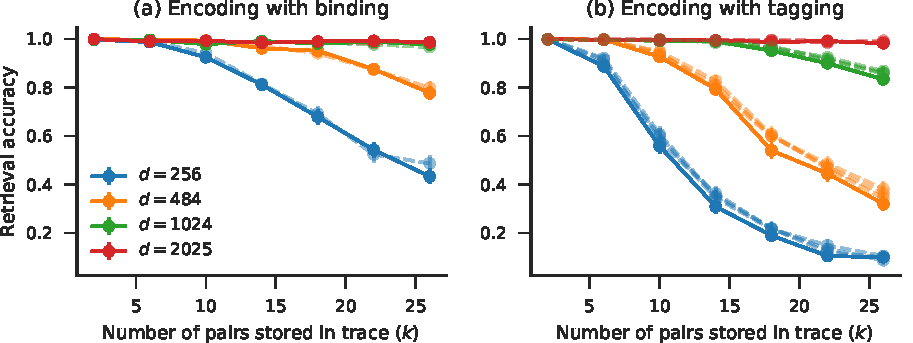
\includegraphics{figures/encoding}
    \caption[Retrieval accuracy of encoding methods]{Retrieval accuracy for (a) encoding with binding and (b) encoding with unitary tagging matrices. Solid lines show results for VTB\@. The dashed lines in (a) show results for binding with circular convolution, in (b) results for unitary circular convolution matrices, shift matrices, and orthogonal matrices without further indication as the results are almost identical. Error bars denote \SI{95}{\percent} confidence intervals.}\label{fig:encoding}
\end{figure}

The results for encoding with tagging by a shift of one are shown in \cref{fig:encoding}b and closely match the results presented in \textcite{recchia2015}.
Note that the same result applies to any other permutation matrix as the vector components can be reordered accordingly.
Very similar results are obtained with orthogonal matrices, fixed unitary circular convolution, and unitary VTB\@.
In all these cases, the pairwise binding capacity is below the encoding with binding, opposed to what \textcite{recchia2015} reported.
Intuitively, this can be explained by the fact that encoding with tagging is a sum of $2k$ vectors, where each vector has encoded information about the pair's constituents, whereas encoding with binding is a sum of $k$ vectors because each pair's constituent gets encoded separately.
In the plots, the retrieval accuracies for encoding with binding at $2k$ matches roughly with the retrieval accuracy with tagging at $k$.
% TODO is this discussion to confusing?

Finally, we can observe (\cref{fig:encoding-nonunitary-tagging}) that encoding with tagging completely fails with fixed non-unitary circular convolution matrices and does not do much better with non-unitary VTB matrices either.
This is likely due to the fact that repeated circular convolution with the same (non-unitary) vector leads to a super-exponential increase in length.
That causes one pair (or even one vector of that pair) to be much stronger than all the other pairs, preventing their recovery.
\begin{figure}
    \centering
    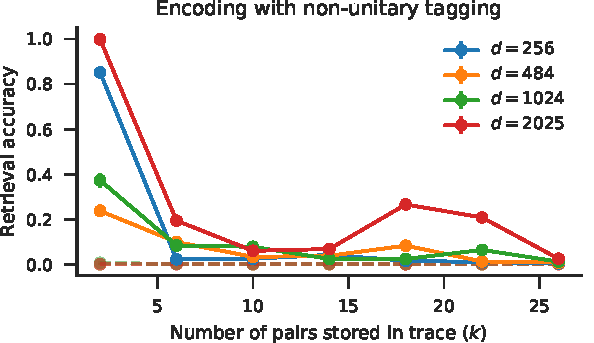
\includegraphics{figures/encoding-nonunitary-tagging}
    \caption[Retrieval accuracy of encoding with non-unitary tagging matrices]{Retrieval accuracy for encoding with non-unitary tagging matrices. Solid lines show results for VTB matrics, while dashed lines show results for circular convolution matrices. Error bars for \SI{95}{\percent} confidence intervals are smaller than then marker size.}\label{fig:encoding-nonunitary-tagging}
\end{figure}

These experiments clearly show that encoding with binding is preferable.
Even more so, as retrieving items from an encoding with tagging is much more involved.
Each potential cue vector $\vc y_i$ has to be recovered and compared to the actual cue $\vc y$ to determine the maximum similarity to the cue, and which $\vc x_i$ has to be decoded from the encoding.
The encoding with binding allows direct querying of an $\vc x_i$ with a given $\vc y_i$.
This makes for a simpler implementation in a neural network.
That being said, if the main concern is not the implementation in a neural network, but the performance of the vector operations on a classical digital computer, one might come to a different conclusion as \textcite{recchia2015} did.
